\chapter{Étude statistique des algorithmes de résolution}\label{annexe_stats}
Le module \texttt{bn\_stats.py} fournit, dans la classe \texttt{Stats}, les outils pour analyser statistiquement une distribution de valeurs (calculs des indicateurs statistiques classiques, représentation en histogramme et diagramme en boîte grâce aux modules \texttt{numpy} et \texttt{matplotlib}).

Cette classe fournit également les outils pour sauvegarder et charger la liste des résultats bruts dans un fichier texte pour des analyses plus poussées futures.

Chaque graphique fait apparaître, outre l'histogramme de distribution des fréquences, les indicateurs suivants :
\begin{itemize}
\item moyenne et écart-type,
\item minimum, $Q_1$, médiane, $Q_3$ et maximum dans le diagramme en boîte,
\item le mode, noté à la base de la barre correspondante,
\item le temps moyen de résolution.
\end{itemize}

\medskip

La méthode de test est la suivante : on crée une liste \texttt{distrib} de longueur \texttt{xmax*ymax+1} qui est initialisée avec des valeurs nulles.\\
On répète $n$ fois la résolution sur une grille aléatoire, chaque fois différente et, en notant $k$ le nombre de coups de la résolution, on incrémente \texttt{distrib[k]} de 1.

\medskip

Le calcul du temps se fait en lançant un chronomètre grâce à la fonction \texttt{time()} du module \texttt{time}, qui renvoie le nombre de seconde écoulées depuis epoch (le 1\up{er} janvier 1970). Donc en sauvegardant cette valeur au début de la simulation dans une variable \texttt{start} et en calculant \texttt{time()-start} à la fin de la simulation, on obtient le temps total écoulé. Afin de chronométrer uniquement le temps de résolution (et non de la création de la grille), ce chronomètre est mis à jour uniquement lors de la résolution effective.

L'algorithme de test, disponible uniquement dans l'interface console, affiche une estimation du temps restant (ainsi que de la date et l'heure de la fin de la simulation) basé sur le temps de la première résolution (donc très approximative), ainsi que l'avancement par tranches de 10\%.

Afin d'obtenir des résultats comparables, tous les temps ont été mesurés sur le même ordinateur disposant d'un processeur Intel i7-4800-MQ cadencé à 2,7 GHz en mode monoprocesseur, de 16 Go de mémoire vive et tournant sous un système Linux 64 bits (Xubuntu 14.04).

%\vfill 
%\begin{flushright}
%Résultats à partir de la page suivante $\rightarrow$
%\end{flushright}
\newpage
\section{Niveau 1}
Dans ce niveau tous les tirs sont aléatoires uniformément sur les cases vides, et il n'y a pas de phase de tirs ciblés.\\
On obtient les résultats suivants sur un échantillon de $n=1\,000\,000$ parties :

\begin{center}
\fbox{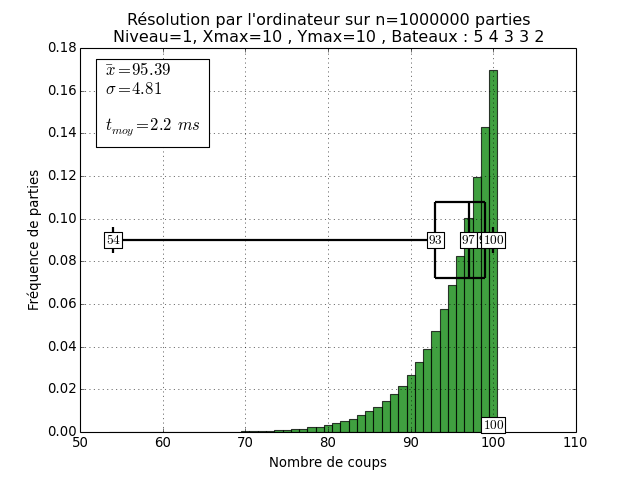
\includegraphics[scale=0.7]{./media/distrib_HAL_niveau=1_n=1000000.png}}
\end{center}

Comme on pouvait s'y attendre, les résultats sont catastrophiques. Par contre la résolution est quasi immédiate (2 ms par partie en moyenne)
\newpage
\section{Niveau 2}
Au niveau 2, la phase de tirs en aveugle est aléatoire uniformément sur les cases vide, mais on ajoute la phase de tirs ciblés lorsqu'on touche un bateau.

Les résultats sur $n=1\,000\,000$ parties sont les suivants :

\begin{center}
\fbox{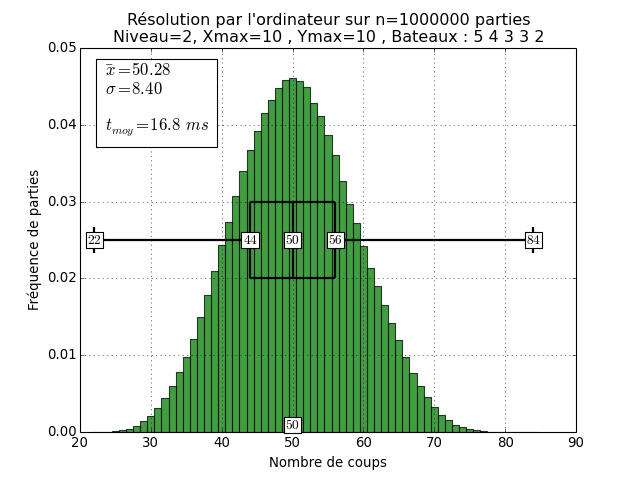
\includegraphics[scale=0.7]{./media/distrib_HAL_niveau=2_n=1000000.png}}
\end{center}

Le fait de gérer la phase de tirs ciblés change radicalement les résultats. La forme de la courbe de distribution est d'ailleurs totalement différente de la précédente.\\
Par contre la résolutions prend 8 fois plus de temps.
\newpage
\section{Niveau 3}
Au niveau 3, la phase de tirs en aveugle est encore aléatoire mais uniquement sur les cases noires.

Les résultats sur $n=100\,000$ parties sont les suivants :

\begin{center}
\fbox{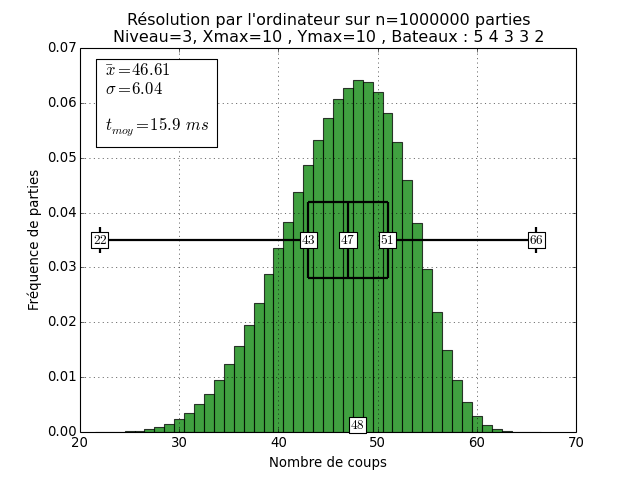
\includegraphics[scale=0.7]{./media/distrib_HAL_niveau=3_n=1000000.png}}
\end{center}

On note une amélioration significative des performances, autant pour la moyenne que pour le mode et la médiane, sans pour autant sacrifier en temps de résolution, au contraire puisqu'il faut moins de coups en aveugle pour finir la grille. Les résultats sont également plus homogènes ($\sigma=6,04$ au lieu de $8,40$ précédemment).

\newpage
\section{Niveau 4}
Au niveau 4 la détermination de la case optimale durant la phase de tirs en aveugle se fait en regardant, à chaque coup, un échantillon de taille \texttt{nb\_echantillons} de distributions de bateau aléatoires.

La valeur de \texttt{nb\_echantillons} va jouer sur les performances en nombre de coups (plus on fait d'échantillons et plus la distribution de probabilités obtenue est conforme à la vraie distribution de probabilité) mais aussi sur le temps de résolution. En effet ce dernier sera linéaire en \texttt{nb\_echantillons}.

Vu le temps de calcul, les simulations suivantes portent sur un nombre plus faible de parties (la contrainte fixée est que le calcul ne doit pas durer plus d'une nuit).
\subsection{Échantillons de taille \texttt{nb\_echantillons=10}}
Avec des échantillons de taille 10 nous obtenons les résultats suivants sur $n=100\,000$ parties :

\begin{center}
\fbox{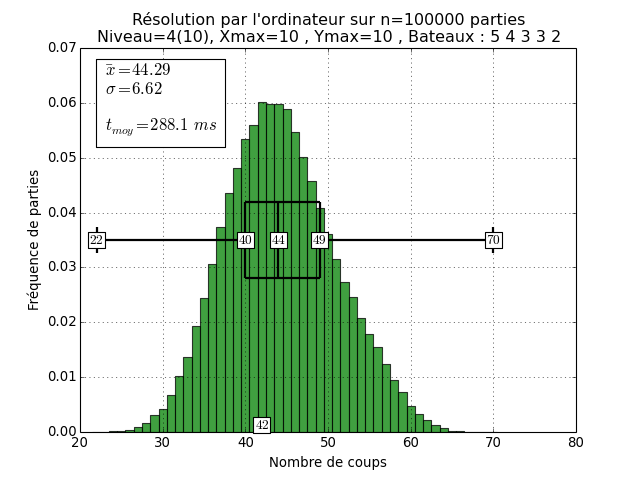
\includegraphics[scale=0.7]{./media/distrib_HAL_niveau=4(10)_n=100000.png}}
\end{center}

Avec une taille modeste des échantillons, nous obtenons une nette amélioration des performances avec une moyenne de 44,29,  pour un temps moyen de 0,3 secondes par partie.
 
\newpage
\subsection{Échantillons de taille \texttt{nb\_echantillons=100}}
Avec des échantillons de taille 100 nous obtenons les résultats suivants sur $n=10\,000$ parties :

\begin{center}
\fbox{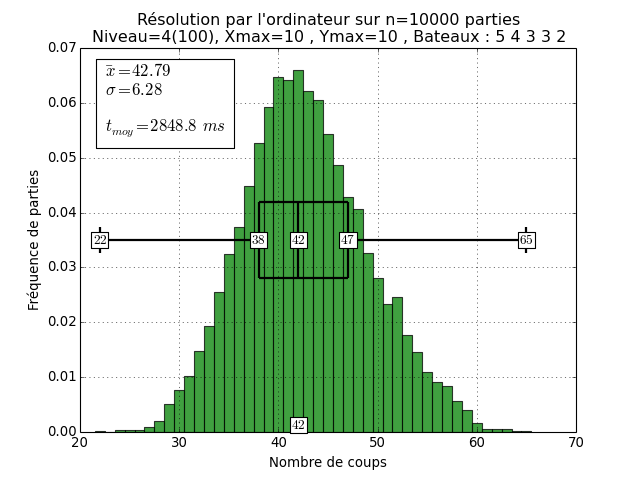
\includegraphics[scale=0.7]{./media/distrib_HAL_niveau=4(100)_n=10000.png}}
\end{center}
 
Les résultats sont très bons, avec une moyenne de 42,84 coups par partie, mais le temps de calcul commence à devenir long (2,5 secondes par partie). 

\newpage
\subsection{Échantillons de taille \texttt{nb\_echantillons=1\,000}}
Nous prévoyons un temps de résolution moyen d'approximativement 30 secondes par partie. Aussi nous ne ferons qu'une simulation sur $n=1\,000$ parties :

\begin{center}
\fbox{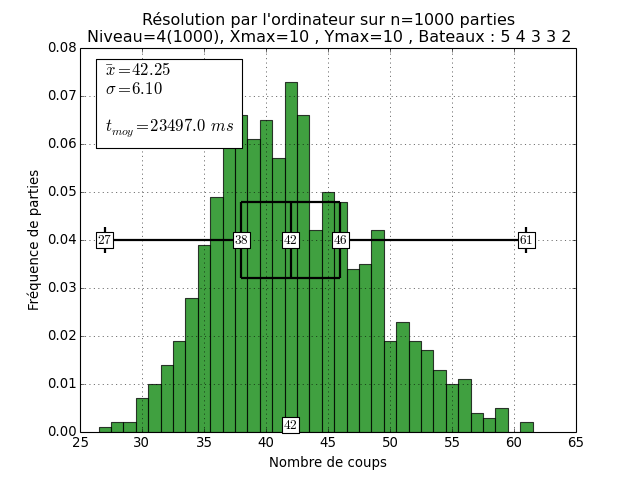
\includegraphics[scale=0.7]{./media/distrib_HAL_niveau=4(1000)_n=1000.png}}
\end{center}

La forme de la distribution est moins régulière que les précédentes à cause du nombre plus réduit de parties simulées.

Le gain en nombre de coups moyen par partie, s'il est présent, est très limité compte tenu de l'augmentation linéaire du temps de calcul. 

\newpage
\subsection{Échantillons de taille \texttt{nb\_echantillons=1\,000}}
Juste pour essayer, voici une simulation sur $n=100$ partie :

\begin{center}
\fbox{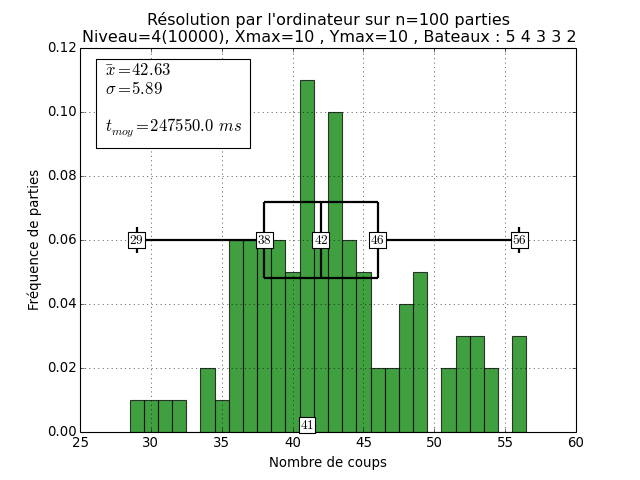
\includegraphics[scale=0.7]{./media/distrib_HAL_niveau=4(10000)_n=100.png}}
\end{center}

Les résultats sont très décevants. On n'a fait que $n=100$ parties ce qui explique peut-être cela mais on note même un régression ce qui est quand même étonnant. 


\newpage
\subsection{Conclusion sur le niveau 4}
Comme on pouvait s'y attendre le temps de résolution est approximativement linéaire en \texttt{nb\_echantillons}.

Les résultats en nombre de coups sont très corrects mais le coût en temps de calcul est rédhibitoire. Par ailleurs, il a été impossible de créer de grosses simulations avec un \texttt{nb\_echantillons} élevé ce qui biaise un peu les comparaisons.

\medskip

Voici un tableau récapitulatif des résultats obtenus :

 \medskip

\begin{center}
\begin{tabular}{|l|c|c|c|c|}
\hline
Numéro de la simulation & 1 & 2 & 3 & 4\\
\hline
Taille des échantillons pour l'algorithme & 10 & 100 &  1\,000 & 10\,000\\
\hline
Nombre de parties $n$ & 100\,000 & 10\,000 & 1\,000 & 100\\
\hline
Nombre de coups moyens $\conj x$ & 44,29 & 42,84 & 42,25 & 42,63\\
\hline
Écart-type\footnote{Vu la taille importante des échantillons nous prendrons $\sigma_\text{estimé}=\sigma_{échantillon}$}  $\sigma$ & 6,62 & 6,24 & 6,10 & 5,89\\
\hline
Temps moyen par partie (en secondes) & 0,29 & 2,5 & 23,5 & 247\\
\hline 
\end{tabular}\\
\end{center}

\medskip

\begin{center}
\begin{tabular}{|l|l|c|}
\hline
\no & \texttt{nb\_echantillons} & Intervalle de confiance\footnote{Au seuil de 95\% : $\left[\conj x-1,96\frac{\sigma}{\sqrt{n}}~;~ \conj x+1,96\frac{\sigma}{\sqrt{n}}\right]$ } de $\mu$ \\
\hline
1 & 10 & $[44,25~;~44,33]$\\
\hline
2 & 100 & $[42,72 ~;~42,96]$\\
\hline
3 & 1\,000 & $[41,87~;~42,63]$\\
\hline
4 & 10\,000& $[41,48~;~43,78]$\\
\hline
\end{tabular}
\end{center}

\newpage
\section{Niveau 5}
Les résultats obtenues sur un échantillon de $n=1\,000\,000$ parties sont les suivants :

\begin{center}
\fbox{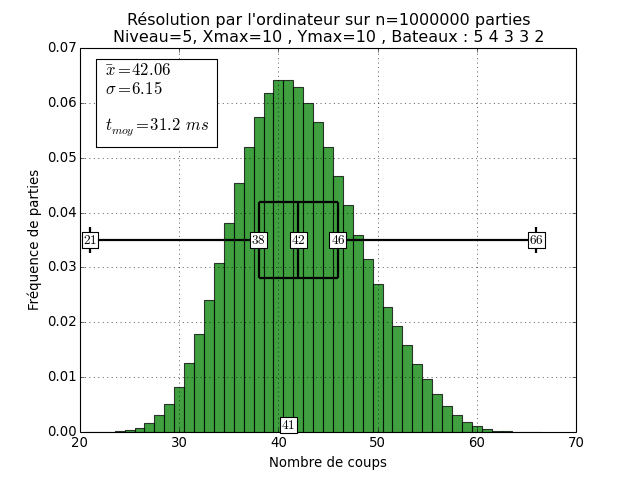
\includegraphics[scale=0.7]{./media/distrib_HAL_niveau=5_n=1000000.png}}
\end{center}

Les performances sont excellentes avec une moyenne de 42,06 coups pour un temps de résolution moyen de seulement 31,2 ms par partie. 

\newpage
\section{Niveau 6}
Au niveau 6, tant que le nombre de cases vides est inférieur à \texttt{seuil}, on procède comme au niveau 5 en regardant localement le nombre de bateaux possibles sur chaque case. Dès que le nombre de cases vides passe en-dessous de \texttt{seuil}, on crée la liste de tous les arrangements possibles de bateaux sur la grille (ce qui prend un temps conséquent, d'où l'obligation d'utiliser un seuil).
\subsection{Seuil égal à 60}
Avec un seuil de 60, les résultats obtenues sur un échantillon de $n=10\,000$ parties sont les suivants :

\begin{center}
\fbox{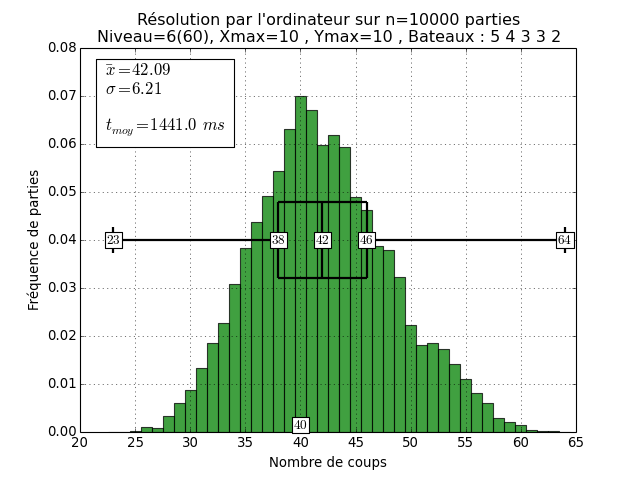
\includegraphics[scale=0.7]{./media/distrib_HAL_niveau=6(60)_n=10000.png}}
\end{center}

Pour l'instant, avec un seuil de 60, nous restons sur notre faim. Il n'y a aucune amélioration par rapport au niveau 5.



\newpage

\subsection{Seuil égal à 70}
Avec un seuil de 70, les résultats obtenues sur un échantillon de $n=1\,000$ parties sont les suivants :

\begin{center}
\fbox{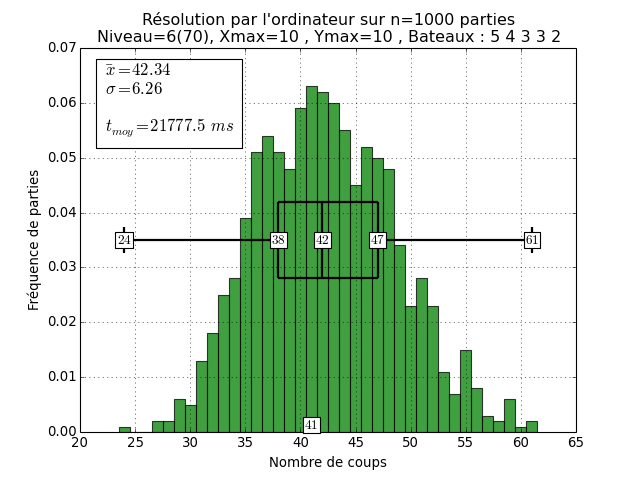
\includegraphics[scale=0.7]{./media/distrib_HAL_niveau=6(70)_n=1000.png}}
\end{center}

À notre grande surprise, la moyenne est un petit peu moins bonne alors qu'on aurait pu imaginer le contraire.

\subsection{Conclusion sur le niveau 6}
Comparons les intervalles de confiance à 95\% de $\mu$ pour les trois dernières simulations :

\begin{center}
\begin{tabular}{|l|l|c|c|c|c|}
\hline
\no & Niveau & $n$ &  $\conj x$ & $\sigma$ & Intervalle de confiance\\
\hline
1 & 5 & 1\,000\,000 & 42,06 & 6,15 & $[42,05~;~42,07]$ \\
\hline
2 & 6(60) & 10\,000 & 42,09 & 6,21 & $[41,97~;~42,21]$\\
\hline
3 & 6(70) & 1\,000 & 42,34 & 6,26 & $[41,95~;~42,73]$\\
\hline
\end{tabular}
\end{center}

C'est un petit peu décevant. On aurait pu prévoir une amélioration du fait de regarder la grille de façon globale. Ce n'est malheureusement pas le cas. Le niveau 5 reste définitivement le meilleur.

\newpage


\section{Conclusions}

Après avoir testé ces différents algorithmes nous pouvons tirer les conclusions suivantes :
\begin{itemize}
\item Le niveau 1 est très médiocre (voire mauvais) mais a l'avantage de la simplicité. On n'a pas à gérer de file d'attente ce qui est pratique dans le cadre d'un projet élève.
\item Le niveau 2 n'a que peu d'intérêt. Il permet uniquement d'introduire la phase de tirs ciblés.
\item Le niveau 3 est, quant à lui, très intéressant. On a une optimisation simple de la phase de tirs en aveugle et des performances tout à fait correctes.
\item Le niveau 4 est intéressant dans le fait qu'il introduit un début d'intelligence artificielle. L'algorithme teste différentes combinaisons avant de prendre sa décision. 
\item Le niveau 5 est de loin le meilleur. L'optimisation est somme toute assez simple pour des résultats qui sont les meilleurs de tous.
\item Le niveau 6 est plus une preuve de concept qu'un algorithme réellement utile en pratique. Les temps de calcul sont pharamineux, ce qui oblige de ne l'utiliser qu'à partir d'un certain moment, et les résultats sont assez décevants par rapport au niveau 5, auquel il n'apporte en fait rien. Il serait toutefois intéressant de le tester (avec un seuil de 100, c'est-à-dire en n'utilisant jamais le niveau 5) en disposant d'une grande puissance de calcul (et de trouver un moyen de paralléliser ceux-ci).
\end{itemize}

\medskip

En tout état de cause il semble qu'une moyenne de 42 coups par partie constitue une borne que l'on ne pourra pas franchir.

%\medskip
%
%À titre de comparaison, ce problème a été étudié par Nick Berry sur son (excellent) blog :
%\begin{center}
%\texttt{http://www.datagenetics.com/blog/december32011/}
%\end{center}
%Par contre il autorise ses bateaux a se toucher sur des cases adjacentes ce que nous avons interdit (et qui permet une résolution plus efficace, mais aussi plus intéressante), ce qui biaise la comparaison. De plus il annonce \og coulé \fg{} lorsqu'un bateau a été coulé. 